%!TEX root = main.tex 
  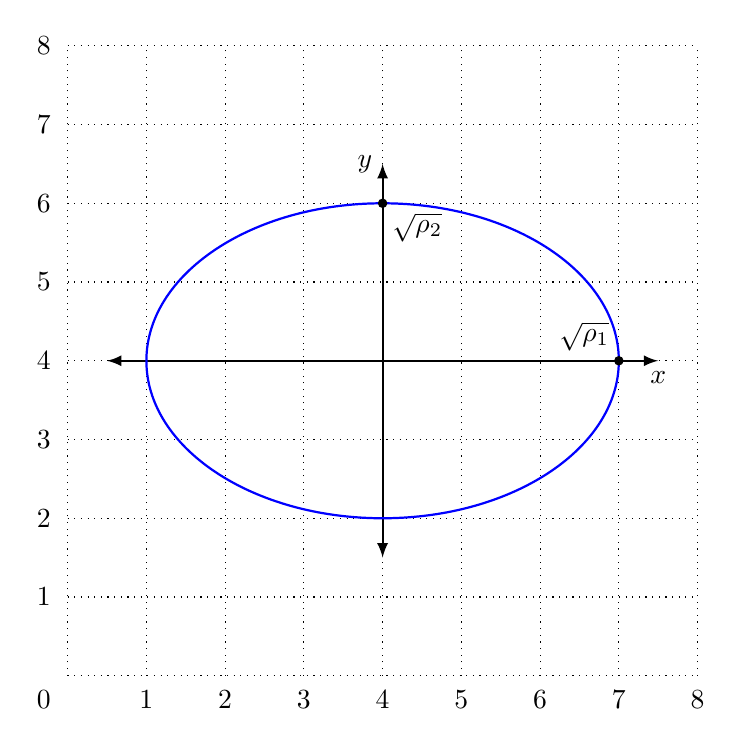
\begin{tikzpicture}
    \draw[thin, dotted] (0,0) grid (8,8);
    \foreach \i in {1,...,8} {
     \node at (\i,-2ex) {\i};  
    }
    \foreach \i in {1,...,8} {
      \node at (-2ex,\i) {\i};  
    }
    \node at (-2ex,-2ex) {0};
    
    \draw[-latex, thick] (4,4) -- (4,6.5) node[left] {$y$};
    \draw[-latex, thick] (4,4) -- (4,1.5) node {};
    \draw[-latex, thick] (4,4) -- (7.5,4) node[below] {$x$};
    \draw[-latex, thick] (4,4) -- (0.5,4) node {};
    
    \draw[blue, thick] (4,4) circle [x radius = 3, y radius = 2];
    \draw[fill=black] (4,6) circle [radius=1.5pt] node[below right] {$\sqrt{\rho_2}$};
    \draw[fill=black] (7,4) circle [radius=1.5pt] node[above left] {$\sqrt{\rho_1}$};
  \end{tikzpicture}
